\subsection{Instrumentos de medición}
\label{sec:instrumentos}

Los equipos empleados se enumeran a continuación; los procedimientos y resultados
de calibración se presentan en la Sección~\ref{sec:procedimientos}.

\subsubsection{Instrumentos de medición dimensional y metrología industrial}
\label{sec:instr-dimensional}

\paragraph{Pie de rey o calibrador vernier}
\label{sec:instr-pie-de-rey}

El pie de rey es un instrumento de medición directa que determina dimensiones
lineales exteriores, interiores y de profundidad. Consta de una regla principal
graduada en milímetros y de un cursor móvil provisto de una escala secundaria o
nonio, que subdivide la menor división de la escala principal y aumenta la
resolución de lectura. El calibrador Mitutoyo Serie 530, código
\mbox{530-115} y número de serie 2013G454, tiene un alcance de $0$ a
$300\ \text{mm}$ y una división de escala de $d = 0{,}05\ \text{mm}$, derivada de
$20$ divisiones del nonio \parencite{mitutoyo_530_115}. La resolución se deduce
de la geometría de la escala en la Sección~\ref{sec:pie-de-rey}. El instrumento
dispone de mordazas rectificadas para medidas exteriores, orejetas superiores
para diámetros interiores y una varilla posterior deslizante para cavidades
profundas. Su calibración se efectuó por comparación directa con bloques patrón
según el procedimiento PC-012 del SNM-INDECOPI \parencite{inacal_pc012}.

\begin{figure}[H]
  \centering
  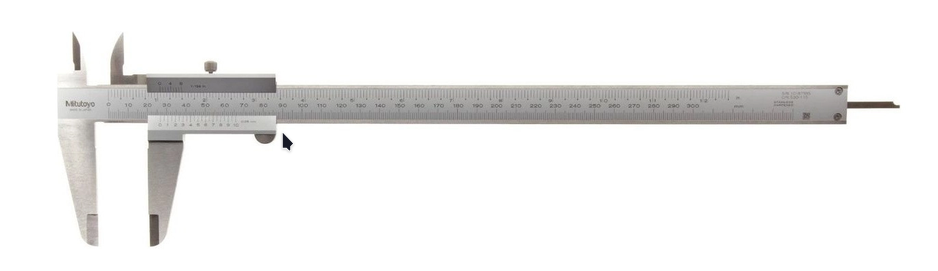
\includegraphics[width=0.55\textwidth]{img/bernier_pie_de_rey.png}
  \caption{Pie de rey Mitutoyo Serie 530, código 530-115.}
  \label{fig:pie-de-rey-instrumento}
\end{figure}

\paragraph{Medidor de profundidad digital}
\label{sec:instr-profundidad}

El medidor de profundidad digital determina la dimensión axial interna de
cavidades, ranuras, escalones y agujeros. Una base plana de apoyo se asienta
sobre la superficie de referencia y un vástago móvil se desplaza
perpendicularmente hasta el fondo del elemento inspeccionado. El medidor INSIZE
de la Serie 1147 tiene resolución de $0{,}01\ \text{mm}$
($0{,}0005''$) y pantalla LCD de lectura directa en milímetros o pulgadas
\parencite{insize_1147_depth}. El equipo dispone de puesta a cero (\texttt{ZERO})
en cualquier posición del recorrido y de conmutación de unidades
(\texttt{mm/inch}), lo que reduce los errores de alineación angular y facilita
la lectura. A diferencia del pie de rey, la base de apoyo no depende de la
posición de las mordazas, por lo que resulta adecuado para cavidades de acceso
restringido.

\begin{figure}[H]
  \centering
  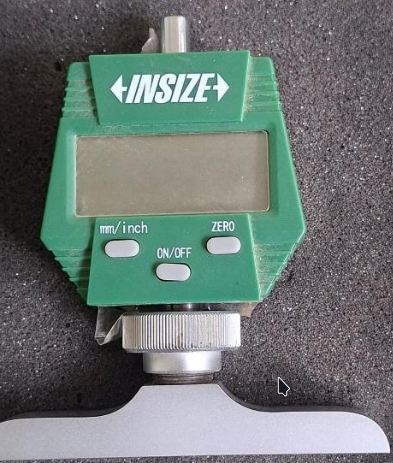
\includegraphics[width=0.30\textwidth]{img/profundidad.png}
  \caption{Medidor de profundidad digital INSIZE Serie 1147, con base de apoyo
  y controles \texttt{ZERO} y \texttt{mm/inch}.}
  \label{fig:profundidad-instrumento}
\end{figure}

\paragraph{Reloj comparador digital}
\label{sec:instr-reloj}

El comparador mide pequeñas desviaciones dimensionales y de forma por
comparación: transforma el desplazamiento axial del palpador en una indicación
de alta resolución. El comparador digital Mitutoyo ID-S1012M, código
\mbox{543-682/543-682B} y número de serie 12038057, tiene un alcance de
$0$ a $12{,}7\ \text{mm}$, una resolución de $0{,}01\ \text{mm}$ y una
exactitud de $\pm 0{,}02\ \text{mm}$ \parencite{mitutoyo_ids1012m}. Se usa en la
verificación de excentricidades, paralelismos y planitudes sobre una mesa de
granito. ISO~463:2006 define la terminología y las características metrológicas
de los comparadores mecánicos de cuadrante; se cita solo como referencia de los
errores de indicación \parencite{iso463_2006}. La calibración se realizó por
comparación con bloques patrón según el procedimiento PC-014 del
INACAL~\parencite{inacal_pc014}, desarrollada en la
Sección~\ref{sec:reloj-comparador}.

\begin{figure}[H]
  \centering
  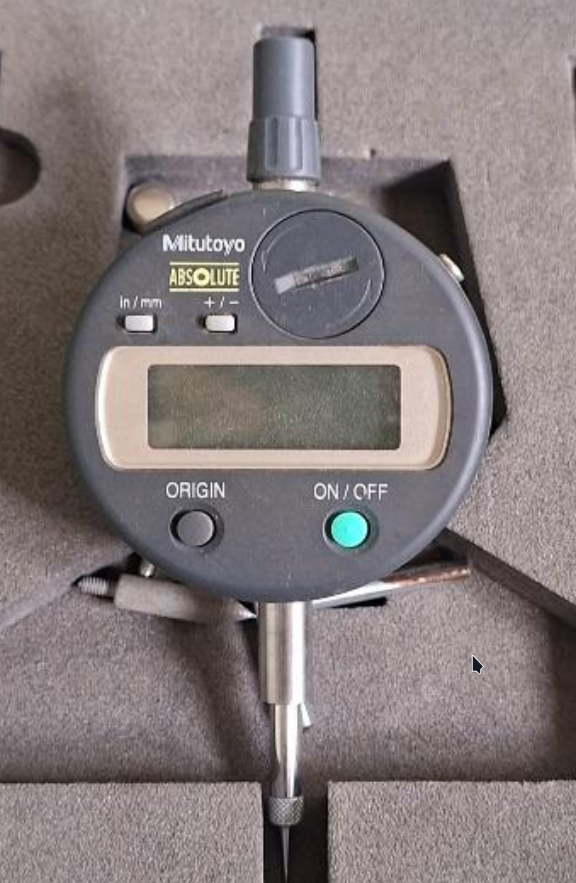
\includegraphics[width=0.30\textwidth]{img/comparator_clock.png}
  \caption{Detalle del comparador digital Mitutoyo ABSOLUTE utilizado en la
  calibración.}
  \label{fig:reloj-instrumento}
\end{figure}

\subsubsection{Equipos y patrones de ultrasonido y acústica}
\label{sec:instr-ut}

\paragraph{Medidor de espesores por ultrasonido}
\label{sec:instr-medidor-ut}

El medidor de espesores por ultrasonido es un equipo de ensayos no destructivos
que determina el grosor de una pared desde un solo acceso, sin alterar la
estructura evaluada. Funciona por el método de eco de pulso: un transductor
emite un impulso ultrasónico que se refleja en la cara posterior y el equipo
mide el tiempo de vuelo $\Delta t$ para calcular $d = c_L\,\Delta t/2$,
relación deducida en la Sección~\ref{sec:ut}
(ecuación~\eqref{eq:espesor-tof}). El medidor INSIZE ISU-100D lleva un
transductor piezoeléctrico de contacto de $5\ \text{MHz}$, un rango de $0{,}8$ a
$300\ \text{mm}$ y una resolución de $0{,}01\ \text{mm}$ \parencite{insize_isu100d}.
Para evitar la atenuación de la onda en la interfaz sonda--pieza se aplica gel
de glicerina como acoplante acústico. La calibración y la verificación de
linealidad se realizaron según el procedimiento PC-029 del
INACAL~\parencite{inacal_pc029} y la práctica ASTM E797~\parencite{astm_e797},
con los resultados recogidos en la Sección~\ref{sec:ut-calibracion}.

\begin{figure}[H]
  \centering
  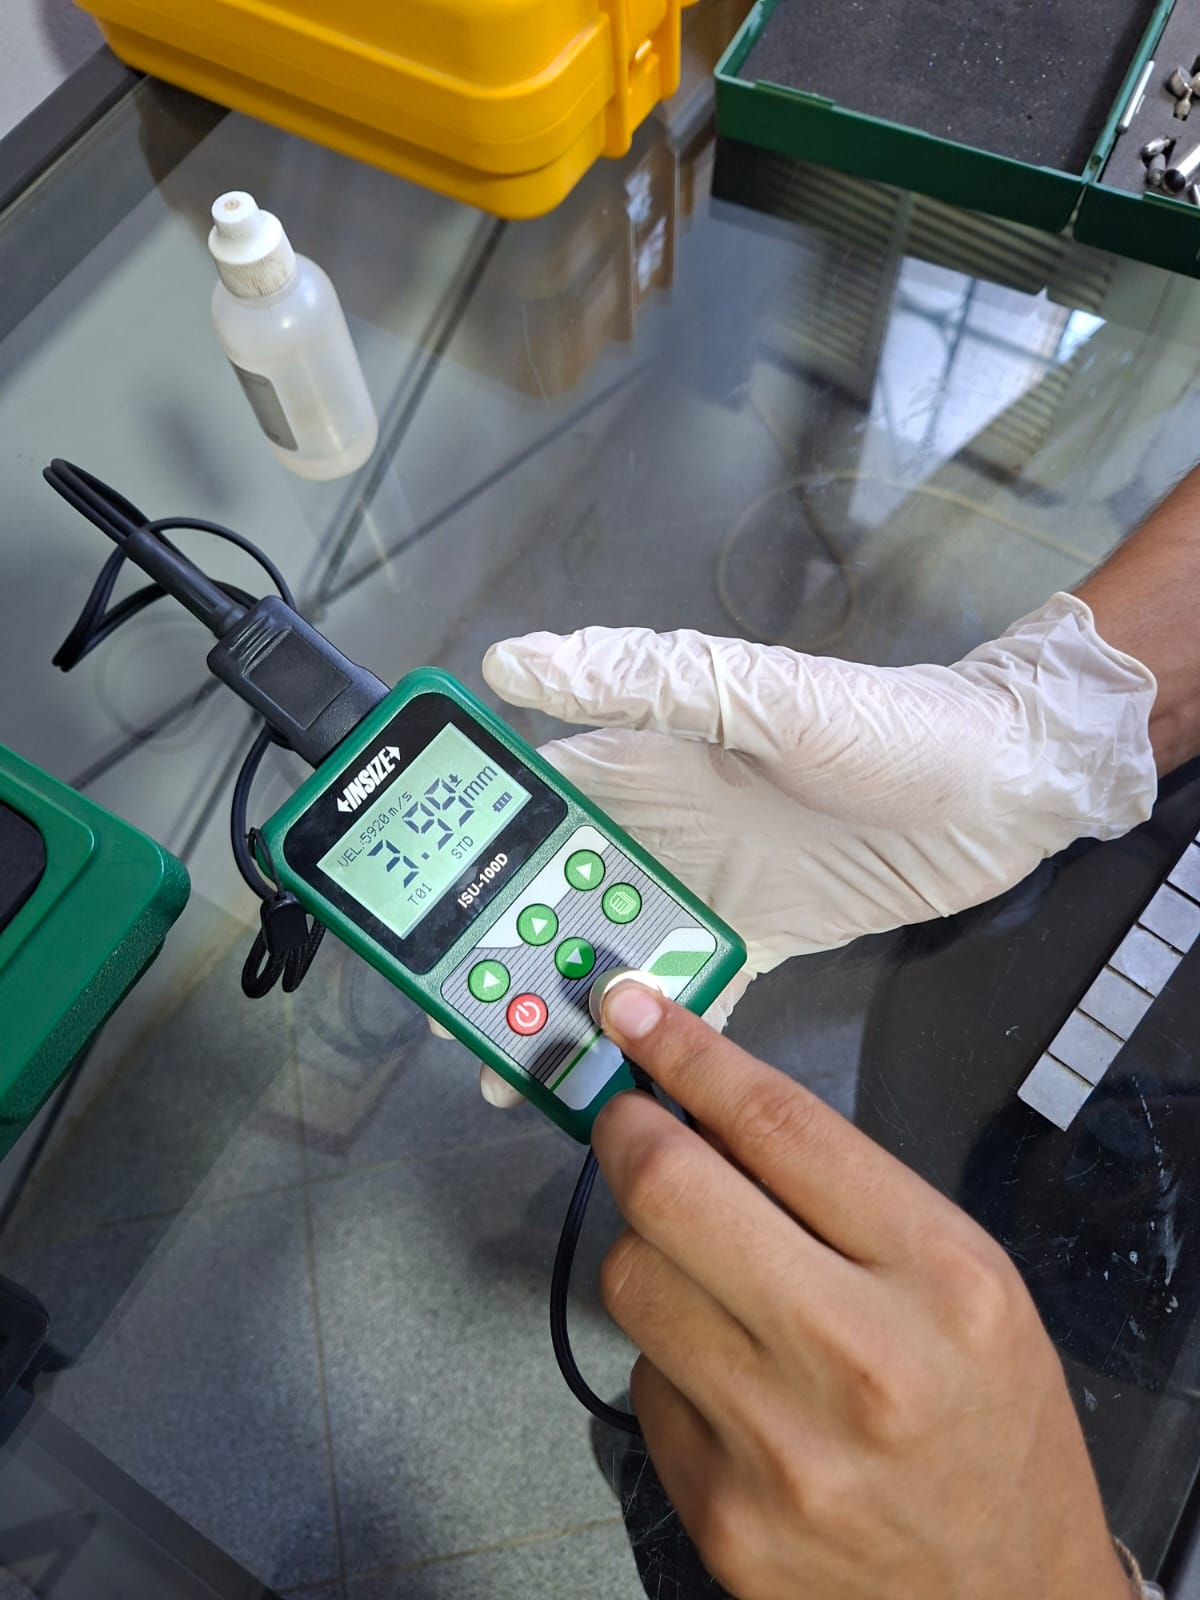
\includegraphics[width=0.42\textwidth]{img/ultrasound_instrument.jpeg}
  \caption{Medidor INSIZE ISU-100D con el transductor de 5 MHz y el acoplante.}
  \label{fig:ut-instrumento}
\end{figure}

\paragraph{Bloque patrón escalonado de espesores}
\label{sec:instr-step-block}

El bloque escalonado es un patrón de referencia empleado para ajustar la
velocidad del sonido, verificar la linealidad de escala y calibrar medidores de
espesores por ultrasonido. Consiste en un bloque de acero con diez niveles de
espesor conocido, de $2{,}50$ a $25{,}00\ \text{mm}$ en pasos de $2{,}50\ \text{mm}$.
Cada escalón permite comprobar la respuesta del transductor en un punto del
rango operativo, de modo que las mediciones de espesor quedan trazadas al patrón
certificado. Su empleo se rige por el procedimiento PC-029 \parencite{inacal_pc029}.

\begin{figure}[H]
  \centering
  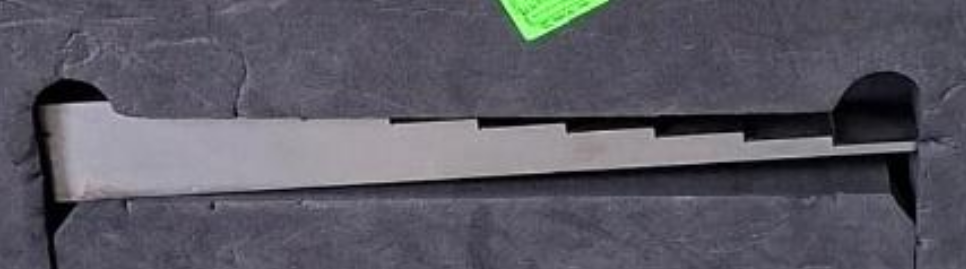
\includegraphics[width=0.55\textwidth]{img/scalonated_block.png}
  \caption{Bloque patrón escalonado de acero, de $2{,}50$ a $25{,}00\ \text{mm}$.}
  \label{fig:step-block-instrumento}
\end{figure}

\subsubsection{Patrones físicos de referencia y trazabilidad metrológica}
\label{sec:instr-bloques}

\paragraph{Bloques patrón de longitud certificados}

Los bloques patrón son estándares prismáticos de longitud, fabricados en acero
de alta estabilidad dimensional, cuyas caras opuestas presentan un pulido plano
de calidad lapidada. Materializan magnitudes fijas con incertidumbres
certificadas y garantizan la cadena de trazabilidad al metro del Sistema
Internacional de Unidades. ISO~3650:1998 especifica sus características
metrológicas y define los grados de exactitud K, 0, 1 y 2 \parencite{iso3650_1998}.
Se emplearon bloques de grado~1 para la calibración del pie de rey y de
grado~2 para el comparador, según se indica en las
Secciones~\ref{sec:pie-de-rey} y~\ref{sec:reloj-comparador}. Las pilas se
conformaron por adherencia capilar (\textit{wringing}) para constituir los
puntos de calibración requeridos en cada alcance.

\begin{figure}[H]
  \centering
  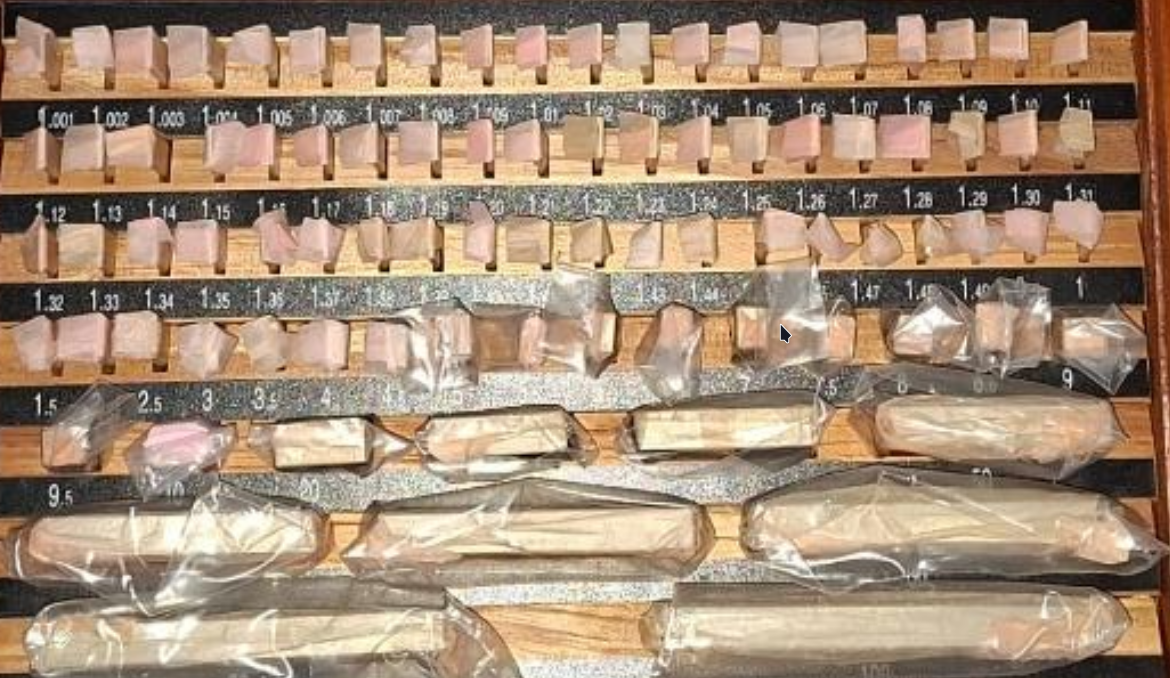
\includegraphics[width=0.55\textwidth]{img/patrones.png}
  \caption{Juego de bloques patrón de longitud.}
  \label{fig:bloques-instrumento}
\end{figure}

\subsubsection{Equipos de ensayos no destructivos para detección de fisuras}
\label{sec:instr-end}

\paragraph{Yugo electromagnético}
\label{sec:instr-yugo}

El yugo electromagnético es un equipo portátil de partículas magnéticas que
localiza discontinuidades superficiales y subsuperficiales en materiales
ferromagnéticos. Una bobina interna montada sobre un núcleo articulado con dos
patas ajustables induce un campo magnético local en la pieza; si una grieta
interrumpe las líneas de campo aparece una fuga de flujo magnético que atrae y
acumula las partículas aplicadas, revelando la falla. El fundamento físico se
desarrolla en la Sección~\ref{sec:mt}. El yugo Magnaflux Y-7 AC/DC tiene por
números de parte actuales 625643 (115~V) y 625644 (230~V); el número
43560 corresponde a una designación anterior del modelo de 230~V
\parencite{magnaflux_y7_yoke}. El modo de corriente alterna se usa para
defectos superficiales y el de corriente continua para fallas subsuperficiales,
conforme a ASTM E1444 e ISO 9934-1 \parencite{astm_e1444, iso9934_1}.

\begin{figure}[H]
  \centering
  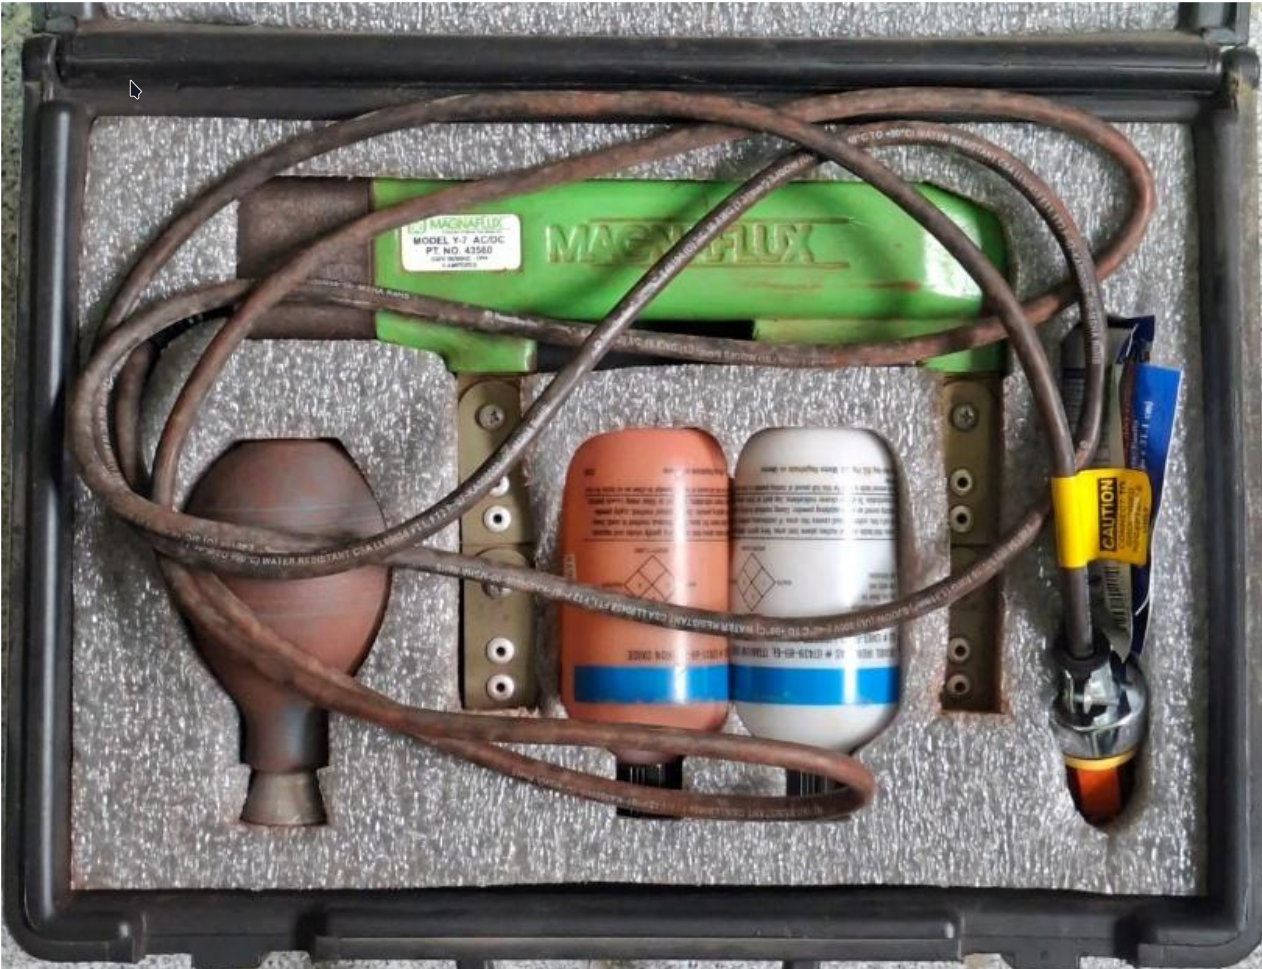
\includegraphics[width=0.45\textwidth]{img/yugo.png}
  \caption{Yugo Magnaflux Y-7 AC/DC (PT 43560) con sus accesorios.}
  \label{fig:yugo-instrumento}
\end{figure}

\paragraph{Lámpara de luz negra (radiación ultravioleta UV-A)}
\label{sec:instr-uv}

La lámpara de luz negra emite radiación UV-A en torno a $\lambda = 365\ \text{nm}$
y se emplea en los ensayos por líquidos penetrantes y partículas magnéticas
fluorescentes. Su función es excitar los pigmentos fotosensibles retenidos en
las fisuras para que emitan fluorescencia verde-amarilla, observable en
condiciones de oscuridad ambiental ($\le 20\ \text{lux}$). La irradiancia
requerida es de al menos $1000\ \mu\text{W/cm}^2$ a $38\ \text{cm}$ de distancia.
ASTM E3022 regula la medición de las características de emisión y los
requerimientos de las lámparas LED UV-A \parencite{astm_e3022_uv}, en tanto que
los criterios de irradiancia e iluminancia para la inspección se establecen en
ASTM E1417 y ASTM E1444 \parencite{astm_e1417, astm_e1444}. La secuencia
operativa se describe en las Secciones~\ref{sec:pt} y~\ref{sec:mt}.

\begin{figure}[H]
  \centering
  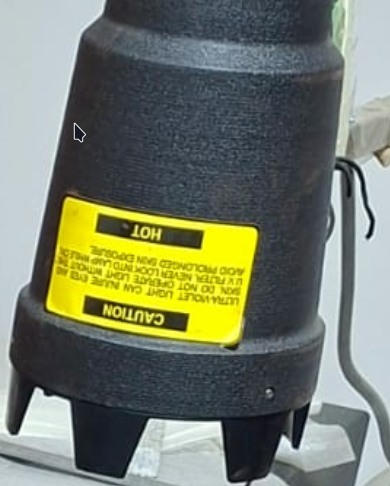
\includegraphics[width=0.30\textwidth]{img/lampara.png}
  \caption{Lámpara UV-A de inspección.}
  \label{fig:uv-instrumento}
\end{figure}
